\documentclass[tikz]{standalone}

\usetikzlibrary{arrows, shapes, positioning}

\begin{document}
    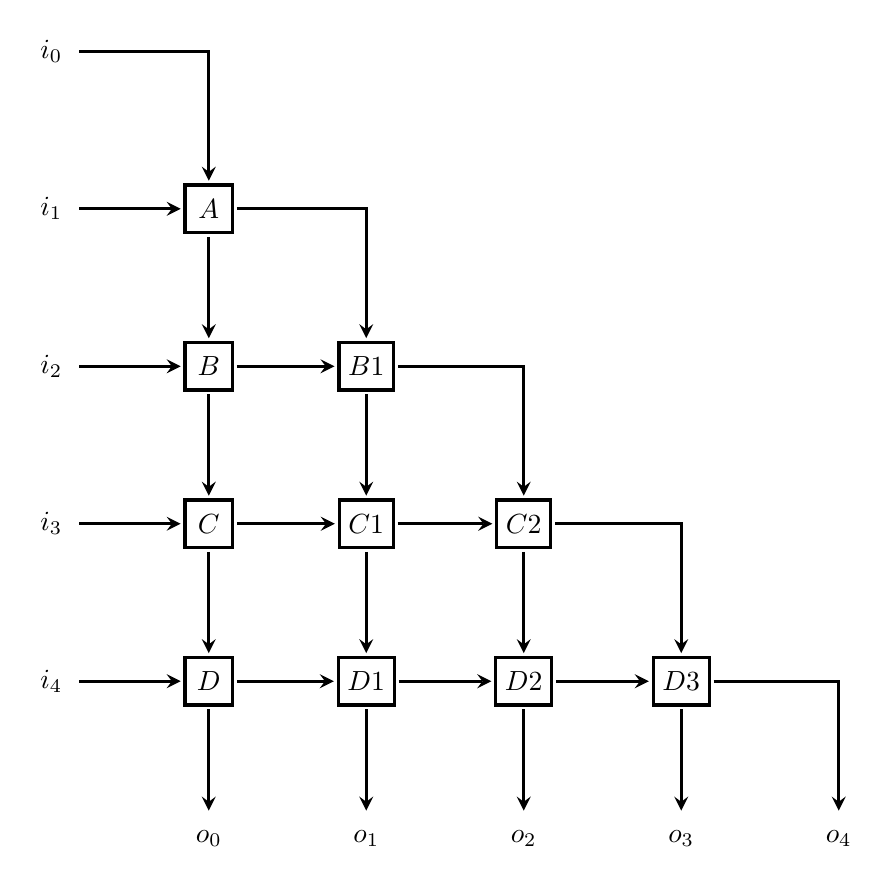
\begin{tikzpicture}[scale=4, >=stealth, node distance=2cm, shorten >=1pt, shorten <=1pt, minimum size=0.6cm, very thick]
        \node[] (i0) {$i_0$};
        \node[below of=i0] (i1) {$i_1$};
        \node[below of=i1] (i2) {$i_2$};
        \node[below of=i2] (i3) {$i_3$};
        \node[below of=i3] (i4) {$i_4$};

        \node[rectangle, draw, right of=i1] (A) {$A$};
        \node[rectangle, draw, below of=A] (B) {$B$};
        \node[rectangle, draw, below of=B] (C) {$C$};
        \node[rectangle, draw, below of=C] (D) {$D$};

        \node[rectangle, draw, right of=B] (B1) {$B1$};
        \node[rectangle, draw, right of=C] (C1) {$C1$};
        \node[rectangle, draw, right of=D] (D1) {$D1$};

        \node[rectangle, draw, right of=C1] (C2) {$C2$};
        \node[rectangle, draw, right of=D1] (D2) {$D2$};

        \node[rectangle, draw, right of=D2] (D3) {$D3$};

        \node[below of=D] (o0) {$o_0$};
        \node[below of=D1] (o1) {$o_1$};
        \node[below of=D2] (o2) {$o_2$};
        \node[below of=D3] (o3) {$o_3$};
        \node[right of=o3] (o4) {$o_4$};

         %Draw horizontal Arrows
        \draw[->] (i0.east) -| (A.north);
        \draw[->] (i1.east) -- (A.west);
        \draw[->] (i2.east) -- (B.west);
        \draw[->] (i3.east) -- (C.west);
        \draw[->] (i4.east) -- (D.west);

        \draw[->] (A.east) -| (B1.north);
        \draw[->] (B.east) -- (B1.west);
        \draw[->] (C.east) -- (C1.west);
        \draw[->] (D.east) -- (D1.west);

        \draw[->] (B1.east) -| (C2.north);
        \draw[->] (C1.east) -- (C2.west);
        \draw[->] (D1.east) -- (D2.west);

        \draw[->] (C2.east) -| (D3.north);
        \draw[->] (D2.east) -- (D3.west);

        % Draw Vertical Arrows
        \draw[->] (A.south) -- (B.north);
        \draw[->] (B.south) -- (C.north);
        \draw[->] (C.south) -- (D.north);

        \draw[->] (B1.south) -- (C1.north);
        \draw[->] (C1.south) -- (D1.north);

        \draw[->] (C2.south) -- (D2.north);

        \draw[->] ( D.south) -- (o0.north);
        \draw[->] (D1.south) -- (o1.north);
        \draw[->] (D2.south) -- (o2.north);
        \draw[->] (D3.south) -- (o3.north);
        \draw[->] ( D3.east) -| (o4.north);

    \end{tikzpicture}
\end{document}
